\documentclass{beamer}
\mode<presentation>
\usepackage[english]{babel}
\usepackage{graphicx}
\usepackage[biolinum]{libertine}

\title{Version control with Git}
\author{Etienne Dysli Metref}
\date{December 2015}

\AtBeginSection[]
{
  \begin{frame}<beamer>{Outline}
    \tableofcontents[currentsection,hideothersubsections]
  \end{frame}
}

\begin{document}
\begin{frame}
  \titlepage
\end{frame}

\begin{frame}{Outline}
  \tableofcontents[hideallsubsections]
\end{frame}

\section{Version control}
\begin{frame}{What is version control?}
  \begin{block}{Record changes made to files over time}
    \begin{itemize}
    \item ``Go back in time'', revert files to previous version
    \item Compare versions, find differences
    \end{itemize}
  \end{block}
  \begin{block}{Collaboration tool}
    \begin{itemize}
    \item Easily share files and changes
    \item Parallel lines of development
    \end{itemize}
  \end{block}
\end{frame}

% \begin{frame}{Centralized vs. distributed}
%   \begin{columns}[t]
%     \begin{column}{6cm}
%       \begin{block}{Centralized}
%         \begin{itemize}
%         \item Examples: CVS, Subversion, Perforce
%         \item Clients check out the latest version from a server
%         \item One place to go
%         \item Single point of failure
%         \end{itemize}
%       \end{block}
%     \end{column}
%     \begin{column}{6cm}
%       \begin{block}{Distributed}
%         \begin{itemize}
%         \item Examples: Git, Mercurial, Bazaar
%         \item Clients check out a complete copy of the repository
%         \item Works without a network connection
%         \item Requires some organization: who is the reference?
%         \end{itemize}
%       \end{block}
%     \end{column}
%   \end{columns}
% \end{frame}

\section{Git concepts}
%reviser def branche/tag
\begin{frame}{Distributed}
  Everyone has a complete copy of the repository
  \begin{center}
    \includegraphics[height=7cm]{images/distributed.png}
  \end{center}
\end{frame}

\begin{frame}{Inside a Git-managed project}
%\texttt{.git} directory is the repository
  \begin{center}
    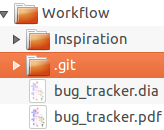
\includegraphics{images/directory_structure.png}
  \end{center}
% \begin{block}{Directory structure}
  % \begin{itemize}
  % \item \texttt{project/} \emph{Working directory}: checkout of a single version of the project
  %   \begin{itemize}
  %   \item \texttt{.git/} Git \emph{repository} storing all data
  %   \item \texttt{fileA} Working copy of files tracked by Git
  %   \item \texttt{fileB}
  %   \item \emph{Staging area (index)}: changes that will go into the next commit
  %   \end{itemize}
  % \end{itemize}
% \end{block}
\end{frame}

\begin{frame}{How Git works}
  \begin{center}
    \includegraphics{images/commit.png}
  \end{center}
  \begin{itemize}
  \item[Commit] Snapshot of files at given time\\No sequential revision numbers but checksums (SHA-1 hash)\\Points to parent commit
  \item[Branch] Pointer to a commit
  \item[Tag] Text label on a commit
  \end{itemize}
\end{frame}

\begin{frame}{Three states}
  \begin{center}
    modified --- staged --- committed
  \end{center}
  \begin{center}
    \includegraphics{images/three_states.png}
  \end{center}
\end{frame}

\begin{frame}{Branching \& merging}
  \begin{center}
    \only<+>{\includegraphics{images/branch0.png}}
    \only<+>{\includegraphics{images/branch1.png}\\New branch ``iss53'' from ``master''}
    \only<+>{\includegraphics{images/branch2.png}\\New commit on branch ``iss53''}
    \only<+>{\includegraphics{images/branch3.png}\\Switch work on new branch ``hotfix''}
    \only<+>{\includegraphics{images/branch5.png}\\Merge ``hotfix'' into ``master'' (fast-forward)\\No conflict}
    \only<+>{\includegraphics{images/branch6.png}\\Merge ``iss53'' into ``master'' (three-way)\\Conflicts can happen}
  \end{center}
\end{frame}

\begin{frame}{Rebasing}{Merging with a cleaner history}
  \begin{center}
    \only<+>{\includegraphics{images/rebase0.png}\\How do we resolve conflicts \emph{before} merging ``experiment'' into ``master''?}
    %\only<+>{\includegraphics{images/rebase1.png}\\Three-way merge}
    \only<+>{\includegraphics{images/rebase2.png}\\Rebase}
    \only<+>{\includegraphics{images/rebase3.png}\\Fast-forward merge}
  \end{center}
\end{frame}

\section{Using Git}
\begin{frame}{Repository creation}
  \only<+>{
    \begin{center}
      \includegraphics{images/tortoise_init.png}
    \end{center}
    \begin{block}{Initializing a repository in an existing directory}
      \texttt{git init}
      \begin{itemize}
      \item Creates the .git directory
      \item But doesn't track any files yet
      \end{itemize}
    \end{block}
  }
  \only<+>{
    \begin{center}
      \includegraphics{images/tortoise_clone.png}
    \end{center}
    \begin{block}{Cloning an existing repository}
      \texttt{git clone <URL>}
      \begin{itemize}
      \item Copies all data from the source repository
      \item Checks out the latest version
      \item Supports several protocols: HTTP, SSH, Git
      \end{itemize}
    \end{block}
  }
\end{frame}

\begin{frame}{Checking in}
\only<+>{
  \begin{center}
    \includegraphics{images/tortoise_add.png}
  \end{center}
  \begin{block}{Staging changes}
    \texttt{git add <file>}
    \begin{itemize}
    \item Adds the current state of the file to version control
    \item Will be in next commit
    %\item Adds the current state of the file to the staging area
    %\item If you modify the file after \texttt{git add}, the \alert{new changes are not staged}.
    \end{itemize}
  \end{block}
}
\only<+>{
  \begin{center}
    \includegraphics{images/tortoise_commit.png}
  \end{center}
  \begin{block}{Committing changes}
    \texttt{git commit}
    \begin{itemize}
    \item Writes every changes in the staging area to the repository
    \item Only staged changes are committed
    \end{itemize}
    % \texttt{git commit -a}
    % \begin{itemize}
    % \item Shortcut: stages and commits all \emph{already tracked} files
    % \end{itemize}
  \end{block}
}
\end{frame}

\begin{frame}{Looking at changes}
  \only<1>{
    \begin{center}
      \includegraphics{images/tortoise_status.png}
    \end{center}
    \begin{block}{Checking the status of your files}
      \texttt{git status}
      \begin{itemize}
      \item Lists files by state
      \item The most useful command to know the current state of your repository
      %\item Gives hints on what to do next or how to undo
      \end{itemize}
    \end{block}
  }
  \only<2-3>{
    \begin{center}
      \includegraphics{images/tortoise_diff.png}
    \end{center}
    \begin{block}{Viewing changes inside files}
      \texttt{git diff}
      \begin{itemize}
      \item Shows what is changed but not yet staged
      \item Compares working directory with staging area
      \end{itemize}
      \onslide<3>
      \texttt{git diff --staged}
      \begin{itemize}
      \item Shows what would go into the next commit
      \item Compares last commit with ``next'' commit
      \end{itemize}
    \end{block}
  }
\end{frame}

% \begin{frame}{Moving files around}
%   \begin{block}<+->{Removing files}
%     \texttt{git rm <file>}
%     \begin{itemize}
%     \item Deletes the file and stages its removal
%     \end{itemize}
%   \end{block}
%   \begin{block}<+->{Renaming files}
%     \texttt{git mv <old name> <new name>}
%     \begin{itemize}
%     \item Renames the file and stages the change
% %    \item Shortcut for three commands:\\\texttt{mv <old name> <new name>\\git rm <old name>\\git add <new name>}
%     \end{itemize}
%   \end{block}
% \end{frame}

\begin{frame}{Ooops! Undoing}
  \only<1-2>{
    \begin{center}
      \includegraphics<1>{images/tortoise_commit.png}
      \includegraphics<2>[width=10cm]{images/tortoise_commit_amend.png}
    \end{center}
    \begin{block}<1-2>{Changing your last commit}
      \texttt{git commit --amend}
      \begin{itemize}
      \item Adds staged files to the last commit
      \item Edit last commit's message
      \end{itemize}
    \end{block}
  }
  \only<3-4>{
    \begin{center}
      \includegraphics{images/tortoise_revert.png}
    \end{center}
    \begin{block}{Unmodifying a modified file}
      \texttt{git checkout -- <file>}
      \begin{itemize}
      \item Discards changes in file
      \item Reverts to last commit
      \end{itemize}
    \end{block}
    \onslide<4>
    \begin{block}{Unstaging a staged file}
      \texttt{git reset HEAD <file>}
      \begin{itemize}
      \item Undo \texttt{git add}
      \end{itemize}
    \end{block}
  }
\end{frame}

\begin{frame}{History}
  \begin{center}
    \includegraphics{images/tortoise_log.png}
  \end{center}
  \begin{block}{Viewing the commit history}
    \texttt{git log}
    \begin{itemize}
    \item Lists commits from most to least recent
    \item Shows commit checksum, author, date and message
    \item Has many options to customise output
    \end{itemize}
  \end{block}
  % \begin{block}<+->{Graphical interface}
  %   \texttt{gitk}
  %   \begin{itemize}
  %   \item Graphical tool to explore commit history
  %   \item Shows list of commits, ancestor graph and commit detail
  %   \end{itemize}
  % \end{block}
\end{frame}

\begin{frame}{Branching and merging}
  \only<+>{
    \begin{center}
      \includegraphics{images/tortoise_branch.png}
    \end{center}
    \begin{block}{Creating a new branch}
      \texttt{git branch <name>}
      \begin{itemize}
      \item Creates a branch from the current branch
      \end{itemize}
    \end{block}
  }
  \only<+>{
    \begin{center}
      \includegraphics{images/tortoise_checkout.png}
    \end{center}
    \begin{block}{Switching to another branch}
      \texttt{git checkout <branch name>}
      \begin{itemize}
      \item Changes working copy files
      \end{itemize}
    \end{block}
  }
  \only<+>{
    \begin{center}
      \includegraphics{images/tortoise_merge.png}
    \end{center}
    \begin{block}{Merging two branches}
      \texttt{git merge <branch name>}
      \begin{itemize}
      \item Merges changes from target branch into current branch
      \item Conflicts can happen
      \end{itemize}
    \end{block}
  }
  \only<+>{
    \begin{center}
      \includegraphics{images/tortoise_rebase.png}
    \end{center}
    \begin{block}{Rebasing}
      \texttt{git rebase <upstream branch>}
      \begin{itemize}
      \item Replays commit on upstream branch
      \end{itemize}
    \end{block}
  }
\end{frame}

\begin{frame}{Interacting with others}
  \only<1>{
    \begin{center}
      \includegraphics{images/tortoise_sync.png}
    \end{center}
    \begin{block}{Linking to remote repositories}
      \texttt{git remote}
      \begin{itemize}
      \item \emph{Remote repositories}: other versions of your project hosted elsewhere
      \item Lists, adds or removes links to remote repositories
        % \item \emph{origin}: link to the repository you cloned from
      \end{itemize}
    \end{block}
  }
  \only<2-3>{
    \begin{center}
      \includegraphics<2>{images/tortoise_fetch.png}
      \includegraphics<3>{images/tortoise_pull.png}
    \end{center}
    \begin{block}{Retrieving updates}
      \only<2>{
        \texttt{git fetch [remote name]}
        \begin{itemize}
        \item Downloads new changes from the remote
        \item Changes go into your repository (\texttt{.git})
        \item Your local work \alert{is not modified}
        \end{itemize}
      }
      \only<3>{
        \texttt{git pull}
        \begin{itemize}
        \item Shortcut: downloads and merges changes
        \item Your local work \alert{is modified}
        \end{itemize}
      }
    \end{block}
  }
  \only<4>{
    \begin{center}
      \includegraphics{images/tortoise_push.png}
    \end{center}
    \begin{block}{Sharing updates}
      \texttt{git push [remote name] [branch name]}
      \begin{itemize}
      \item Sends your changes to a remote repository
      \item \alert{Do not use without arguments}, it pushes everything!
      \end{itemize}
    \end{block}
  }
\end{frame}

\begin{frame}{Where is the manual?}
  \begin{columns}
    \begin{column}[t]{6cm}
      \begin{block}{\emph{Pro Git} book}
        \begin{itemize}
        \item \url{http://git-scm.com/book}
        \item Chapters 1--3
        \end{itemize}
      \end{block}
      \begin{block}{More}
        \begin{itemize}
        \item \url{http://git-scm.com/doc}
        \item Reference
        \item Videos
        \end{itemize}
      \end{block}
    \end{column}
    \begin{column}[t]{3cm}
      \begin{center}
        \includegraphics[height=3cm]{images/pro-git.jpg}
      \end{center}
    \end{column}
  \end{columns}
\end{frame}

\section{Branch layout}
\begin{frame}{Distributed but centralised}
  \begin{center}
    \includegraphics[height=8cm]{images/distributed-origin.png}
  \end{center}
\end{frame}

\begin{frame}{Permanent public branches}
  \begin{columns}
    \begin{column}{6cm}
      \begin{center}
        \includegraphics[height=8cm]{images/git_branches_permanent.pdf}
      \end{center}
    \end{column}
    \begin{column}{5cm}
      \begin{block}<+->{master}
        \begin{itemize}
        \item Production code
        \item Commit $=$ release
        \end{itemize}
      \end{block}
      \begin{block}<+->{development}
        \begin{itemize}
        \item Next release
        \item Always buildable 
        \end{itemize}
      \end{block}
      \begin{block}<+->{support}
        \begin{itemize}
        \item Old releases
        \end{itemize}
      \end{block}
    \end{column}
  \end{columns}
\end{frame}

\begin{frame}{Temporary public branches}
  \begin{columns}
    \begin{column}{6cm}
      \begin{center}
        \includegraphics[height=8cm]{images/git_branches_temporary.pdf}
      \end{center}
    \end{column}
    \begin{column}{5cm}
      \begin{block}<+->{release}
        \begin{itemize}
        \item Preparation of production release
        \item Bug fixes \alert{only}
        \end{itemize}
      \end{block}
      % \begin{block}{support-release}
      %   \begin{itemize}
      %   \item Releases for old versions
      %   \end{itemize}
      % \end{block}
      \begin{block}<+->{hotfix}
        \begin{itemize}
        \item Urgent bug fix
        \end{itemize}
      \end{block}
    \end{column}
  \end{columns}
\end{frame}

\begin{frame}{Temporary private branches}
  \begin{columns}
    \begin{column}{6cm}
      \begin{center}
        \includegraphics[height=8cm]{images/git_branches_private.pdf}
      \end{center}
    \end{column}
    \begin{column}{5cm}
      \begin{block}{feature}
        \begin{itemize}
        \item Separate every feature or bug fix into its own branch
        \item Integrate often (daily) with development branch
        \end{itemize}
      \end{block}
    \end{column}
  \end{columns}
\end{frame}

%\begin{frame}{Daily workflow}
%  Synchronizing your development branch:
%  \begin{enumerate}
%  \item \texttt{git fetch}
%  \item \texttt{git rebase}
%  \item If there are conflicts, fix them, then:
%  \item \texttt{git add} modified files
%  \item \texttt{git rebase --continue}
%  \item \texttt{git push origin development}
%  \end{enumerate}
%  Commit more changes or push to origin
%\end{frame}

\section{Hands-on}

\begin{frame}{Integration with other tools}
  \begin{block}{Redmine}
    Recognizes commit messages containing keywords
    \begin{itemize}
    \item refs, references, IssueID, Issue-Id
    \item fixes, closes, resolves
    \end{itemize}
    followed by an issue number \#123
  \end{block}
  \begin{block}{IDEs}
    \begin{itemize}
    \item Netbeans: built-in from version 7.1
    \item Eclipse: EGit plugin for versions 3.5.2+
    \end{itemize}
  \end{block}
\end{frame}
\end{document}
